\subsection{Single-Point Crossover}
The selection operation generates pool of eligible progenitors as a subset of the current
generation. Randomly selected chromosomes from this 'mating pool' then undergo a
reproductive cycle where alleles are exchanged and offspring are created. This sharing of
genetic information is the vehicle by which fit individuals propagate their beneficial
traits. However, this operation only preserves genetic diversity within the current
generational genotype. There is no new genetic information introduced since only an
exchange of currently available alleles occurs. Thus, if the objective solution does not
exist as some permutation of the currently available genotype, then the crossover
operation will fail to realize the optimal chromosome regardless of the number of
generations.

A great deal of research has been done regarding the mechanism of exchange between two
chromosomes during crossover. Recall that the problem space is fully characterized by the
objective function and that the medium of evaluation is the application specific
chromosome. Prudent design dictates that the structure of the chromosomes is driven
largely by the nature of the objective function. By extension, the optimal process and
manner of allele exchange between chromosomes is an indirect function of problem space
complexity.

For some applications, it may be necessary to carefully regulate which alleles may be
exchanged. These regulations are dictated by the relationships, if any, which exist
between adjacent groups of alleles. However, there is a fine balance between preserving
the stochastic nature of reproduction and the unintended deterministic exchange of
genetic information. The power of evolutionary strategies lies in achieving balance
between exploration of the solution space and exploitation of the localized minima or
maxima. Thus, the structure of the chromosome (which is representative of the problem
space) should be complementary to the crossover method selected.

Single-point crossover has been selected for this application. Single-point
crossover does have positional bias in that it favors continuous segments of genetic
information. However, it does not contain distribution bias as the crossover point is a
discrete random variable with uniform distribution over $\bigl[0,m\bigr]$, where $m$
denotes the length of the respective chromosome\cite{glover_handbook_2003}. Recall that
the alleles represent the coefficients of first and second order polynomials. Thus, there
is no reason to govern the genetic exchange. Further, any exchanges which violate the
underlying algebra will be reflected in the evaluated fitness of the progeny and will be
short lived.

Once the progenitors have been selected, the crossover point is established. All alleles
subsequent to the crossover point are exchanged between the progenitors and two progeny
are created. The single-point crossover process is illustrated in Figure
\ref{fig:crossover} where the progenitor chromosomes are denoted as $\mathcal{C}_x$ and
the progeny chromosomes are denoted as $\mathcal{C}_x^\prime$.
%----------------------------
\begin{figure}[htbp]
\centering
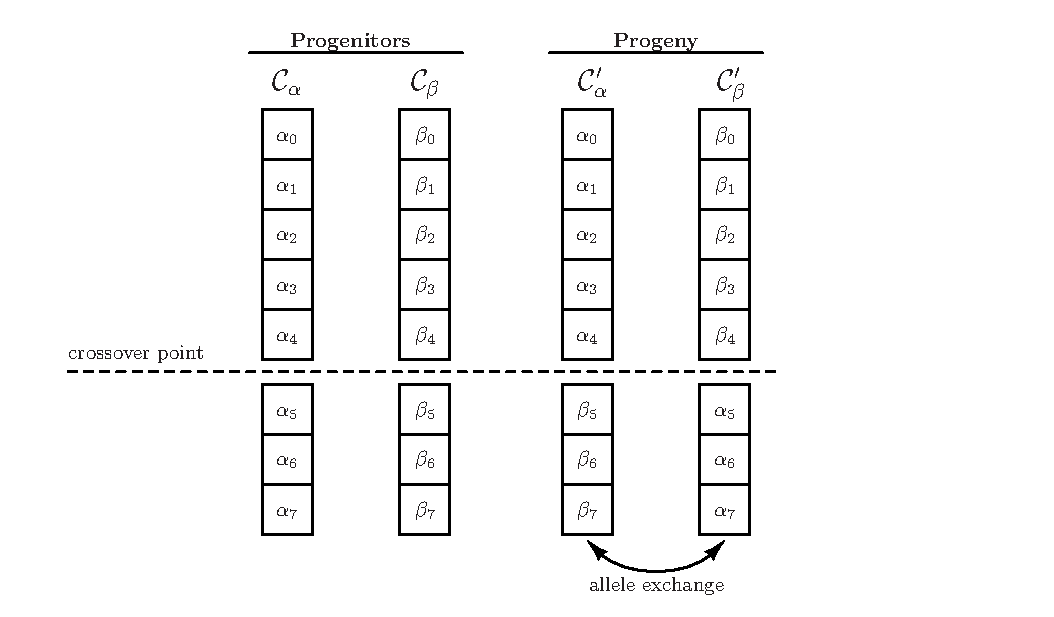
\includegraphics[width=\textwidth]{./final_figures/crossover.eps}
\caption{Single-Point Crossover}
\label{fig:crossover}
\end{figure}
%----------------------------

The process by which individuals are randomly selected is also typically regulated. For
this application, self replication is strictly forbidden. Thus, selected individuals must
crossover with a different individual thereby ensuring the exchange of alleles. This
prevents a single anomalous individual from inadvertently dominating the greater
population which can lead to premature convergence.